\documentclass{vldb}
\usepackage{graphicx}
\usepackage{balance}

\usepackage{color}
\usepackage[noend]{algpseudocode}
\usepackage{algorithm}
\usepackage{varwidth}
\usepackage{url}
\usepackage{multirow}
\usepackage{subfigure}
\usepackage{mathtools}
\usepackage{amsmath,bm}
\usepackage{hyperref}

\usepackage{times}

\renewcommand{\arraystretch}{1.18}

\newtheorem{definition}{Definition}
\newtheorem{variant}{Variant}
\newtheorem{problem}{Problem}
\newtheorem{example}{Example}
\newtheorem{lemma}{Lemma}
\newtheorem{proposition}{Proposition}

\newcommand{\fang}[1]{{\color{red}[\textbf{Yixiang:} #1]}}
\newcommand{\rey}[1]{{\color{blue}[\textbf{Reynold:} #1]}}
\newcommand{\luo}[1]{{\color{purple}[\textbf{Siqiang:} #1]}}
\newcommand{\hu}[1]{{\color{green}[\textbf{Jiafeng:} #1]}}

\newcommand{\tabincell}[2]{\begin{tabular}{@{}#1@{}}#2\end{tabular}}

\begin{document}

%\title{Label-Aware Community Search on Attributed Graphs}

\title{Effective Community Search for Large Attributed Graphs}
\numberofauthors{1}
\author{
\alignauthor \text{ } Authors\\
       \affaddr{Department of Computer Science, The University of Hong Kong, Pokfulam Road, Hong Kong}\\
       \email{\{authors\}@cs.hku.hk}
}

\maketitle
\begin{abstract}
Given a graph $G$ and a vertex $q \in G$, the {\it community search} query returns a subgraph of $G$ that contains vertices related to $q$. Communities, which are prevalent in {\it attributed graphs} such as social networks and knowledge bases, can be used in emerging applications such as product advertisement and setting up of social events.
In this paper, we investigate the {\it attributed community query} (or ACQ), which returns an {\it attributed community} (AC) for an {\it attributed graph}. The AC is a subgraph of $G$, which satisfies both {\it structure cohesiveness} (i.e., its vertices are tightly connected) and {\it keyword cohesiveness} (i.e., its vertices share common keywords).  The AC enables a better understanding of how and why a community is formed (e.g., members of an AC have a common interest in music, because they all have the same keyword ``music'').  An AC can be ``personalized''; for example, an ACQ user may specify that an AC returned should be related to some specific keywords like ``research'' and ``sports''.

To enable efficient AC search, we develop the CL-tree index structure and three algorithms based on it. We further propose efficient algorithms for maintaining the index on dynamic graphs. Moreover, we study two problems that are related to the ACQ problem. We evaluate our solutions on six large graphs. Our results show that ACQ is more effective and efficient than existing community retrieval approaches. Moreover, an AC contains more precise and personalized information than that of existing community search and detection methods. 
\end{abstract}

%\category{H.2.8}{Database Management}{Database Applications}[Data mining]
%\category{G.2.2}{Discrete Mathematics}{Graph Theory}[Graph algorithms]

\section{Introduction}
\label{intro}

Due to the recent developments of gigantic social networks (e.g., Flickr, Facebook, and Twitter), the topic of {\it attributed graphs} has attracted attention from industry and research communities~\cite{attr-topic-sigmod2012,keyword-icde2002,keyword-icde2007,keyword-sigmod2007,keyword-vldb2005,keyword-yu-2009,keyword-vldb2011,fang2014}.  An attributed graph is essentially a graph associated with text strings or keywords.  Figure~\ref{fig:motivation} illustrates an attributed graph, where each vertex represents a social network user, and its keywords describe the interest of that user.

\begin{figure}
	\small
	\centering
	\includegraphics[width=0.88\linewidth]{figures/motivation}
	\caption{Attributed graph and AC (circled).}
	\label{fig:motivation}
\end{figure}

In this paper, we investigate the {\it attributed community query} (or ACQ). Given an attributed graph $G$ and a vertex $q \in G$, the ACQ returns one or more subgraphs of $G$ known as {\it attributed communities} (or ACs).  An AC is a kind of {\it community}, which consists of vertices that are closely related~\cite{KDD2010,local2014,online-sigmod2013,k-truss2014,community-phy2004,community-phy2010}.  Particularly, an AC satisfies {\it structure cohesiveness} (i.e., its vertices are closely linked to each other) and {\it keyword cohesiveness} (i.e., its vertices have keywords in common). Figure~\ref{fig:motivation} illustrates an AC (circled), which is a connected subgraph with vertex degree 3; its vertices $\{${\tt Jack}, {\tt Bob}, {\tt John}, {\tt Mike}$\}$ have two keywords (i.e., ``research'' and ``sports'') in common.

{\bf Prior works.} %An AC is a kind of {\it community}.
The problems related to retrieving communities from a graph can generally be classified into {\it community detection} (CD) and {\it community search} (CS).  In general, CD algorithms aim to retrieve all communities for a graph~\cite{community-phy2004,community-phy2010,attr-vldb2009,attr-topic-kdd2008,attr-topic-icml2009,attr-topic-sigmod2012,attr-www2013,yang2013community}. These solutions are not ``query-based'', i.e., they are not customized for a query request (e.g., a user-specified query vertex).
%For example, it is not clear how these algorithms can return a community that contain a given vertex $q$.
Moreover, they can take a long time to find all the communities for a large graph, and so they are not suitable for quick or {\it online} retrieval of communities. To solve these problems, CS solutions have been recently developed~\cite{KDD2010,local2014,online-sigmod2013,k-truss2014,huang2015approximate,barbieri2015efficient}. These approaches are query-based, and are able to derive communities in an ``online'' manner. However, existing CS algorithms assume {\it non-attributed} graphs, and only use the graph structure information to find communities. The ACQ is a class of CS problem for attributed graphs. As we will show, the use of keyword information can significantly improve the effectiveness of the communities retrieved. Table~\ref{tab:method} summarizes some representative existing works in this area.

\begin{table}
  \centering \footnotesize \caption {Classification of works in community retrieval. }\label{tab:method}
  \begin{tabular}{c|c|c}
     \hline
        \tabincell{c}{\textbf{Graph}\\ \textbf{Type}}
                       & \tabincell{c}{\textbf{Community}\\ \textbf{detection (CD)}}
                       & \tabincell{c}{\textbf{Community}\\ \textbf{search (CS)}}\\
     \hline\hline
        Non-attributed & \cite{community-phy2004,community-phy2010}
                       & \cite{KDD2010,local2014,online-sigmod2013,k-truss2014,vldb2015,huang2015approximate}\\
     \hline
        Attributed     & \cite{attr-vldb2009,attr-topic-kdd2008,attr-topic-icml2009,attr-topic-sigmod2012,attr-www2013,yang2013community}
                       & {\bf ACQ}\\
     \hline
  \end{tabular}
\end{table}

{\bf Features of ACs.} We now present more details of ACs.

\noindent $\bullet$ {\bf Ease of interpretation.}
As demonstrated in Figure~\ref{fig:motivation}, an AC contains tightly-connected vertices with similar contexts or backgrounds. Thus, an ACQ user can focus on the common keywords or features of these vertices (e.g., the vertices of the AC in this example contain ``research'' and ``sports'', reflecting that all members of this AC like research and sports).  We call the set of common keywords among AC vertices
the \emph{AC-label}. In our experiments, the AC-labels facilitate understanding of the vertices that form the AC.

The design of ACs allows it to be used in setting up of social events. For example, if a Twitter member has many keywords about traveling (e.g., he posted a lot of photos about his trips, with keywords), issuing an ACQ with this member as the query vertex may return other members interested in traveling,  because their vertices also have keywords related to traveling. A group tour can then be recommended to these members.

\noindent $\bullet$ {\bf Personalization.}  The user of an ACQ can control the semantics of the AC, by specifying a set of $S$ of keywords. Intuitively, $S$ decides the meaning of the AC based on the user's need.  If we let $q$={\tt Jack}, $k$=2 and $S$=$\{$``research''$\}$,  the AC is formed by
$\{${\tt Jack}, {\tt Bob}, {\tt John}, {\tt Mike}, {\tt Alex}$\}$, who are all interested in research.
Let us consider another example in the DBLP bibliographical network, where each vertex's attribute is represented by the top-20 frequent keywords in their publications. Let $q$={\tt Jim} {\tt Gray}. If $S$ is the set of keywords \{transaction, data, management, system, research\}, we obtain the AC in Figure~\ref{fig:jim}(a), which contains six prominent database researchers closely related to Jim. On the other hand, when $S$ is \{sloan, digital, sky, survey, SDSS\}, the ACQ yields another AC in Figure~\ref{fig:jim}(b), which indicates the seven scientists involved in the SDSS project~\footnote{URL of the SDSS project: \url{http://www.sdss.org}.}.  Thus, with the use of different keyword sets $S$, different ``personalized'' communities can be obtained.

Existing CS algorithms, which do not handle attributed graphs, may not produce the two ACs above. For example, the CS algorithm in \cite{KDD2010} returns the community with {\it all} the 14 vertices shown in Figures~\ref{fig:jim}(a) and (b). The main reasons are: (1) these vertices are heavily linked with Jim; and (2) the keywords are not considered. In contrast, the use of set $S$ in the ACQ places these vertices into two communities, containing vertices that are cohesive in terms of {\it structure} and {\it keyword}. This allows a user to focus on the important vertices that are related to $S$. For example, using the AC of Figure~\ref{fig:jim}(a), a database conference organizer can invite speakers who have a close relationship with Jim.

The personalization feature is also useful in marketing. Suppose that Mary, a yoga lover, is a customer of a gym. An ACQ can be issued on a social network, with Mary as the query vertex and $S$=$\{$``yoga''$\}$. Since members of the AC contain the keyword ``yoga'', they can be the gym's advertising targets. On the other hand, current CS algorithms may return a community that contains one or more vertices without the keyword ``yoga''. It is not clear whether the corresponding user of this vertex is interested in yoga.

\noindent $\bullet$ {\bf Online evaluation.}  Similar to other CS solutions, we have developed efficient ACQ algorithms for large graphs, allowing ACs to be generated quickly upon a query request. On the contrary, existing CD algorithms~\cite{attr-vldb2009,attr-www2013,attr-topic-kdd2008,attr-topic-icml2009} that generate all communities for a graph are often considered to be offline solutions, since they are often costly and time-consuming, especially on very large graphs.

{\bf Technical challenges and our contributions.}
We face two important questions: (1) What should be a sound definition of an AC? (2) How to evaluate ACQ efficiently?  For the first question, we define an AC based on the {\it minimum degree}, which is one of the most common structure cohesiveness metrics~\cite{community-phy2004,community-phy2010,KDD2010,local2014}. This measure requires that every vertex in the community has a degree of $k$ or more.
%one of the most fundamental characteristics of graphs, and some recent works~\cite{KDD2010,local2014} have shown that it is better than many other metrics like average degree and density of a graph.
We formulate the keyword cohesiveness as maximizing the number of shared keywords in keyword set $S$. The shared keywords naturally reveal the common features among vertices (e.g., common interest of social network users). We can also use these shared keywords to explain how a community is formed.

\begin{figure}[ht]
    \centering
    \mbox{
        \subfigure[$S$=\{transaction, data, management, system, research\}]{
            \includegraphics[width=.44\columnwidth]{figures/jim1}
            \label{fig:jim1}
        }
        \hspace{1ex}
        \subfigure[$S$=\{sloan, digital, sky, data, sdss\}]{
            \includegraphics[width=.432\columnwidth]{figures/jim2}
            \label{fig:jim2}
        }
    }
    \caption{Two ACs of Jim Gray.}\label{fig:jim}
\end{figure}

The second question is not easy to answer, because the attributed graph $G$ to be explored can be very large, and the (structure and keyword) cohesiveness criteria can be complex to handle. A simple way is first to consider all the possible keyword combinations, and then return the subgraphs, which satisfy the minimum degree constraint and have the most shared keywords. This solution, which requires the enumeration of all the subsets of $q$'s keyword set, has a complexity exponential to the size $l$ of $q$'s keyword set. In our experiments, for some queries, $l$ can be up to 30, resulting in the consideration of $2^{30}=1,073,741,824$ subsets of $q$. The algorithm is impractical, especially when $q$'s keyword set is large.

{\color{blue}
We observe the {\it anti-monotonicity} property, which states that given a set $S$ of keywords, if it appears in every vertex of an AC, then for every subset $S'$ of $S$, there exists an AC in which every vertex contains $S'$. We use this intuition to propose better algorithms. We further develop the \emph{CL-tree}, an index that organizes the vertex keyword data in a hierarchical structure. The CL-tree has a space and construction time complexity linear to the size of $G$.
Based on the CL-tree index, we have developed three different ACQ algorithms, and they are able to achieve a superior performance.
In practice, graphs are continuously evolving \cite{chenghui,kddEvolving}. For instance, in the friendship network of Facebook, users may change their profiles, and make new friends or remove friendship. Thus the CL-tree index needs to be updated to reflect the changes in the graph. A straightforward method to handle the update is to rebuild the CL-tree from scratch. However, this can be very computationally expensive, especially when the updates are very frequent. To alleviate this issue, we have developed efficient algorithms to maintain the CL-tree index for dynamic graphs.

In addition, we have proposed two typical variants of the ACQ problem, which are called {\it Approximate ACQ problem} (or ACQ-A) and {\it Multiple-vertex ACQ problem} (or ACQ-M) respectively.
ACQ-A is an approximation version of the ACQ query, in which vertices of an AC do not need to exactly share the same keywords as that in ACQ. It relaxes the constraint on sharing common keywords; this could be very useful if vertices of the graph do not have much keyword information.
ACQ-M generalizes the ACQ query for supporting multiple query vertices. It takes multiple query vertices as input and returns the ACs containing all of them. This could be very helpful if we want to find the ACs for a group of query vertices. For example, a database workshop organizer may be interested in inviting researchers who have a close relationship with both Jim Gray and Michael Stonebraker.
To answer the queries for ACQ-A and ACQ-M, we have also developed efficient algorithms based on the CL-tree index.
}

We have performed extensive experiments on six large real graph datasets.
We found that a large number of common keywords appear across vertices in our graph datasets. In DBLP, for instance, an AC with one common keyword contains over 5,000 vertices on average; an AC with two common keywords contains over 700 vertices. Hence, using shared keywords among vertices as keyword cohesiveness makes sense.
We have also studied how to quantify the quality of a community, based on occurrence frequencies of keywords and similarity between the keyword sets of two vertices. We conducted a detailed case study on DBLP. These results confirm the superiority of the AC over the communities returned by existing community detection and community search algorithms, in terms of community quality. The performance of our best algorithm is 2 to 3 order-of-magnitude faster than solutions that do not use the CL-tree.
We have also experimentally evaluated the index maintenance algorithms and the results show that they are very efficient.
Moreover, we perform the queries of the ACQ-A and ACQ-M problems, and the results show that our index-based algorithms are much faster than the baseline algorithms. In addition, our approaches achieve a higher efficiency than existing community search solutions (that do not use vertex keywords in the community search process).

{\bf Organization.} We review the related work in Section~\ref{related}, and define the ACQ problem formally in Section~\ref{problem}. Section~\ref{basic} presents the basic solutions, and Section~\ref{index} discusses the CL-tree index.
In Section~\ref{indexMaintenance}, we discuss how to maintain the CL-tree index for dynamic graphs.
We present the query algorithms in Section~\ref{query}.
In Section~\ref{variant}, we introduce two variants and the corresponding query algorithms.
Our experimental results are reported in Section~\ref{experiment}.
We conclude in Section~\ref{conclusion}. 

\section{Related Work}
\label{related}

%We now discuss two main classes of community retrieval solutions. We also summarize the graph keyword search solutions for attributed graphs.

\textbf{Community detection (CD).} A large class of studies aim to discover or {\it detect} all the communities from an entire graph. Table~\ref{tab:method} summarises these works. Earlier solutions, such as \cite{community-phy2004,community-phy2010}, employ link-based analysis to obtain these communities. However, they do not consider the textual information associated with graphs. Recent works focus on attributed graphs, and use clustering techniques to identify communities.
%Clustering is a typical way to discover communities.
For instance, Zhou et al.~\cite{attr-vldb2009} considered both links and keywords of vertices to compute the vertices' pairwise similarities, and then clustered the graph.
Ruan et al.~\cite{attr-www2013} proposed a method called {\tt CODICIL}. This solution augments the original graphs by creating new edges based on content similarity, and then uses an effective graph sampling to boost the efficiency of clustering. We will compare ACQ with this method experimentally.

Another common approach is based on topic models. In~\cite{attr-topic-kdd2008,attr-topic-icml2009}, the {\tt Link-PLSA-LDA} and {\tt Topic-Link LDA} models jointly model vertices' content and links based on the {\tt LDA} model. In~\cite{attr-topic-sigmod2012}, the attributed graph is clustered based on probabilistic inference. In~\cite{attr-topic-www2012}, the topics, interaction types and the social connections are considered for discovering communities. {\tt CESNA}~\cite{attr-icdm2013} detects overlapping communities by assuming communities ``generate'' both the link and content. A discriminative approach~\cite{attr-kdd2009} has also been considered for community detection. As discussed before, CD algorithms are generally slow, as they often consider the pairwise distance/similarity among vertices.
Also, it is not clear how they can be adapted to perform online ACQ. In this paper, we propose online algorithms for finding communities on attributed graphs.

\textbf{Community search (CS).}  Another class of solutions aims to obtain communities in an ``online'' manner, based on a query request. For example, given a vertex $q$, several existing works~\cite{KDD2010,local2014,vldb2015,online-sigmod2013,k-truss2014} have developed fast algorithms to obtain a community for $q$.
To measure the structure cohesiveness of a community, the {\it minimum degree} is often used~\cite{KDD2010,local2014,vldb2015}. Sozio et al.~\cite{KDD2010} proposed the first algorithm {\tt Global} to find the $k$-$\widehat{core}$ containing $q$.
Cui et al.~\cite{local2014} proposed {\tt Local}, which uses local expansion techniques to enhance the performance of {\tt Global}. We will compare these two solutions in our experiments.
Other definitions, including $k$-clique~\cite{online-sigmod2013} and $k$-truss~\cite{k-truss2014}, have also been considered for searching communities. A recent work~\cite{vldb2015} finds communities with high influence.  These works assume non-attributed graphs, and overlook the rich information of vertices that come with attributed graphs. As we will see, performing CS on attributed graphs is better than on non-attributed graphs.

\textbf{Graph keyword search.}  Given an attributed graph $G$ and a set $Q$ of keywords, graph keyword search solutions output a tree structure, whose nodes are vertices of $G$, and the union of these vertices' keyword sets is a superset of $Q$~\cite{keyword-icde2002,keyword-icde2007,keyword-vldb2005}. Recent work studies the use of a subgraph of $G$ as the query output~\cite{keyword-vldb2011}. These works are substantially different from the ACQ problem. First, they do not specify query vertices as required by the ACQ problem. Second, the tree or subgraph produced do not guarantee structure cohesiveness. Third, keyword cohesiveness is not ensured; there is no mechanism that enforces query keywords to be shared among the keyword sets of all query output's vertices. Thus, graph keyword search solutions are not designed to find ACs.

%{\color{red}
%\textbf{Graph pattern matching (GPM).}  Given a {\it pattern} $P$, the goal of GPM is to extract a set $R$ of subgraphs of $G$, where for every $r \in R$, $r$ is highly similar to $P$.
%Tong et al.~\cite{GPM-KDD2007} studied the use of lines, loops and stars; Fan et al.~\cite{GPM-VLDB2010,GPM-SIGMOD2011} proposed bounded simulation techniques for GPM queries;
%in \cite{GPM-PVLDB2015}, GPM has been studied for finding association rules from graphs.
%However, there is no detailed study about how to use GPM for community search.
%}

%Older version: July 12, 2016
%\textbf{Graph pattern matching (GPM).}  Given a {\it pattern} $P$, the goal of GPM is to extract a set $R$ of subgraphs of $G$, where for every $r \in R$, $r$ is highly similar to $P$.
%Tong et al.~\cite{GPM-KDD2007} studied the use of lines, loops and stars; Fan et al.~\cite{GPM-VLDB2010,GPM-SIGMOD2011} proposed bounded simulation techniques for GPM queries;
%in \cite{GPM-PVLDB2015}, GPM has been studied for finding association rules from graphs.
%However, there is no detailed study about how to use GPM for community search.  To do this, a user has to define $P$, but this is not trivial: there are many possible topologies for $P$, and numerous ways of placing keywords on the vertices in $P$.  Moreover, current GPM solutions focus on small patterns that generate small communities, and it is not clear whether they can support large and complex ones. Answering ACQ with GPM can also be expensive, since it involves enumerating many patterns and finding an AC with the largest number of shared keywords.  For the ACQ problem, there is no need to specify $P$.


\clearpage
\section{The PCQ problem}
\label{PCQproblem}




\begin{definition}[$k$-core~\cite{md1983,kcore2003}]
\label{def:kcore}
Given an integer $k$ ($k\geq 0$), the $k$-core of $G$,
denoted by $H_{k}$, is the largest subgraph of $G$, such that $\forall v \in H_k$, $deg_{H_k}(v) \geq k$.
\end{definition}

\begin{definition}[Profile-tree]
xxxx
\end{definition}

\begin{definition}[Induced rooted subtree]
Given two P-trees $T$ and $S$ rooted at $r_t$ and $r_s$. $T$ is the induced rooted subtree of $S$ iff there exist a one-to-one mapping $\varphi$: $V_s \to V_t$ and $l$ denotes the label of tree node $x$, three constraints hold:

\vspace{1ex}

$\bullet$ $\varphi(r_s)=r_t$;

$\bullet$ $\forall x \in V_s$, $l(x)=l(\varphi(x))$;

$\bullet$ $\forall (x,y) \in E_s$, $(\varphi(x),\varphi(y)) \in E_t$. 
\end{definition}

{\it Inuduced rooted subtree} preserves the parent-child relationships as well as corresponding labels. In addition, the root node of the trees must be preserved. Unless otherwise specified, all uses of the term ``subtree'' refer to ``induced rooted subtree''. P-trees $T$ and $S$ are {\it isomorphic} iff $T$ is the subtree of $S$ and $S$ is the subtree of $T$ simultaneously.


\begin{definition}[Maximum common subtree]
Given a graph $G$, $D$ is a P-tree database which pairs with vertices in $G$. $T$ is the common subtree of $D$ such that $\forall t \in D$, $T$ is the subtree of $t$. Furthermore, $T$ is the maximum common subtree of $D$ (denoted as $\Gamma(G)$) if there exists no other common subtree $T'$ such that $T$ is the subtree of $T'$. 

%Given a graph $G_{\sigma}$, $D_{\sigma}$ is a P-tree database which pairs with vertices in $G_{\sigma}$. $|D_{\sigma}|=\sigma$. 
%T$ is the maximum $\sigma$-common subtree in $G_{\sigma}$ iff $\forall t \in D_{\sigma}$, $T$ is the subtree of $t$ and there exists no other common subtree $T'$ in $D_{\sigma}$ such that $T$ is the subtree of $T'$.
\end{definition}



\begin{problem}[PCQ]
\label{PCQ}
Given a profiled graph $G(V,E)$, a profile tree $T$, a positive integer $k$, and one query node $q\in G$, find a set $\mathcal {G}$ of graphs, such that $\forall G_q \in \mathcal {G}$, the following properties hold:

\vspace{1ex}

$\bullet$ \textbf{Connectivity cohesiveness}. (1)$G_q \subseteq G$ is connected and contains $q$, (2)$\forall v\in G_q$, $deg_{G_q}(v)\geq k$;

$\bullet$ \textbf{Maximal structure}. There exists no other $\tilde G_q$ satisfying \textbf {connectivity cohesiveness} such that $G_q \subset \tilde G_q$ if $\Gamma(G_q)$ and $\Gamma(\tilde G_q)$ are isomorphic;

$\bullet$ \textbf{Semantic cohesiveness}. There exists no other $\tilde G_q$ satisfying \textbf {connectivity cohesiveness}, such that $\Gamma(G_q)$ is the subtree of $\Gamma(\tilde G_q)$.

\end{problem}

\input{basic}

\input{index}

\section{Query Algorithms}
\label{query}

In this section, we present three query algorithms based on the CL-tree index.
Based on how we verify the candidate keyword sets, we divide our algorithms into incremental algorithms (from examining smaller candidate sets to larger ones) and decremental algorithm (from examining larger candidate sets to smaller ones).
We propose two incremental algorithms called \textbf{{\tt Inc-S}} (\underline{Inc}remental \underline{S}pace efficient) and \textbf{{\tt Inc-T}} (\underline{Inc}remental \underline{T}ime efficient), to trade off between the memory consumption and the computational overhead.
The decremental algorithm is called \textbf{{\tt Dec}} (\underline{Dec}remental).
Our interesting finding is that, while {\tt Dec} seems not intuitive, it ranks as the most efficient one.
{\tt Inc-S} and {\tt Inc-T} are presented in Section~\ref{inc}.
{\tt Dec} is introduced in Section~\ref{dec}.

\input{query1}
\input{query2} 

\section{Experiments}
\label{experiment}

We now present the experimental results. Section~\ref{setup} discusses the setup. We discuss the results in Sections~\ref{effectiveness} and \ref{efficiency}. \chen{The experimental results of variants are presented in Sections~\ref{app:varExp}.}

\subsection{Setup}
\label{setup}

We consider six real datasets. The first four datasets (Flickr, DBLP, Tencent, and DBpedia) are static graphs.
For {\it Flickr}~\footnote{\url{https://www.flickr.com/}}~\cite{thomee2015new}, a vertex represents a user, and an edge denotes a ``follow'' relationship between two users. For each vertex, we use the 30 most frequent tags of its associated photos as its keywords.
For {\it DBLP}~\footnote{\url{http://dblp.uni-trier.de/xml/}}, a vertex denotes an author, and an edge is a co-authorship relationship between two authors.
For each author, we use the 20 most frequent keywords from the titles of her publications as her keywords.
In the {\it Tencent} graph provided by the KDD contest 2012~\footnote{\url{http://www.kddcup2012.org/c/kddcup2012-track1}}, a vertex is a person, an organization, or a microblog group. Each edge denotes the friendship between two users. The keyword set of each vertex is extracted from a user's profile. For the {\it DBpedia}~\footnote{\url{http://dbpedia.org/datasets}}, each vertex is an entity, and each edge is the relationship between two entities. The keywords of each entity are extracted by the Stanford Analyzer and Lemmatizer.
Table~\ref{tab:dataset} shows the number of vertices and edges, the $k_{max}$ value, a vertex's average degree $\widehat d$, and its keyword set size $\widehat l$.

{\color{blue}
The remaining two dynamic datasets,
i.e., {\it DFlickr} and {\it Youtube}~\cite{mislove-2009-socialnetworksthesis,mislove-2008-flickr},
are dynamic evolving graphs, which contain the snapshots of graphs as the time goes on.
Note that these two datasets do not have keywords.
Both DFlickr and Youtube datasets are about the user friendship networks on Flickr and Youtube websites respectively.
Each vertex denotes a user and each edge denotes a friendship between two users.
DFlickr contains edges which are inserted and deleted during the evolving process;
while in Youtube, there are only inserted edges as the time goes on.
}

\begin{table}[h]
  \centering
  \small
  \footnotesize \caption {Datasets used in our experiments.}\label{tab:dataset}
  \begin{tabular}{c|r|r|c|c|c}
     \hline
          {\bf Dataset}  & \multicolumn{1}{c|}{\textbf{Vertices}}
                         & \multicolumn{1}{c|}{\textbf{Edges}}
                         & $k_{max}$
                         & \textbf{\emph{{$\widehat d$}}}
                         & \textbf{\emph{{$\widehat l$}}}\\
     \hline\hline
          Flickr         &  581,099      &  9,944,548   &   152   & 17.1   &  9.90 \\
     \hline
          DBLP           &  977,288      &  3,432,273   &   118   &  7.02  &  11.8 \\
     \hline
          Tencent        &  2,320,895    &  50,133,369  &   405   &  43.2  &  6.96 \\
     \hline
          DBpedia        &  8,099,955    &  71,527,515  &    95   &  17.7  &  15.0 \\
     \hline
          DFlickr        &  2,585,569    &  45,676,553  &   600   &  17.6  &  --- \\
     \hline
          Youtube        &  1,881,147    &  9,142,046   &   55   &  4.9  &  --- \\
     \hline
  \end{tabular}
\end{table}

{\color{blue}
To evaluate ACQs, we set the default value of $k$ to 6. The input keyword set $S$ is set to the whole set of keywords contained by the query vertex. For each dataset, we randomly select 300 query vertices with core numbers of 6 or more, which ensures that there is a $k$-core containing each query vertex.
Each data point is the average result for these 300 queries.

To evaluate the index maintenance algorithms, we consider all the six datasets.
For the first four datasets, we randomly select 1,000 vertices and for each of them, we randomly insert and delete one keyword to evaluate the perform keyword update. Meanwhile, we randomly insert and delete five groups of edges, each of which has 100 edges, and their core numbers vary from 5 to 25.
For each of the remaining datasets (DFlickr and Youtube), we first take the snapshots in 100 consecutive days, then divide them into five groups, each of which are in a period of 20 consecutive days, and finally we randomly select 200 records from each group as test edges.
}

We implement all the algorithms in Java, and run experiments on a machine having a quad-core Intel i7-3770 3.40GHz processor, and 32GB of memory, with Ubuntu installed.
We present the effectiveness and efficiency results in Sections~\ref{effectiveness} and~\ref{efficiency}.


\input{effectiveness}

\subsection{Results on Efficiency}
\label{efficiency}

\begin{figure*}[htp]
\hspace*{-.4cm}
\centering
\begin{tabular}{c c c c}
  \begin{minipage}{3.76cm}
	\includegraphics[width=3.725cm]{figures/flickr-index}
  \end{minipage}
  &
  \begin{minipage}{3.76cm}
	\includegraphics[width=3.725cm]{figures/dblp-index}
  \end{minipage}
  &
  \begin{minipage}{3.76cm}
	\includegraphics[width=3.725cm]{figures/tencent-index}
  \end{minipage}
  &
  \begin{minipage}{3.76cm}
	\includegraphics[width=3.725cm]{figures/dbpedia-index}
  \end{minipage}
  \\
  \small (a) Flickr (scalability)
  &
  \small (b) DBLP (scalability)
  &
  \small (c) Tencent (scalability)
  &
  \small (d) DBpedia (scalability)
\end{tabular}
\caption{Efficiency results of index construction.}
\label{fig:exp-index}
\end{figure*}



\begin{figure*}[htp]
\hspace*{-.4cm}
\centering
\begin{tabular}{c c c c}
  \begin{minipage}{3.76cm}
  \includegraphics[width=3.725cm]{figures/flickrUpdate}
  \end{minipage}
  &
  \begin{minipage}{3.76cm}
  \includegraphics[width=3.725cm]{figures/dblpUpdate}
  \end{minipage}
  &
  \begin{minipage}{3.76cm}
  \includegraphics[width=3.725cm]{figures/tencentUpdate}
  \end{minipage}
  &
  \begin{minipage}{3.76cm}
  \includegraphics[width=3.725cm]{figures/dbpediaUpdate}
  \end{minipage}
  \\
  \small (a) Flickr (index maint.)
  &
  \small (b) DBLP (index maint.)
  &
  \small (c) Tencent (index maint.)
  &
  \small (d) DBpedia (index  maint.)
  \\
 \begin{minipage}{3.76cm}
  \includegraphics[width=3.725cm]{figures/flickrMix}
  \end{minipage}
  &
  \begin{minipage}{3.76cm}
  \includegraphics[width=3.725cm]{figures/dblpMix}
  \end{minipage}
  &
  \begin{minipage}{3.76cm}
  \includegraphics[width=3.725cm]{figures/tencentMix}
  \end{minipage}
  &
  \begin{minipage}{3.76cm}
  \includegraphics[width=3.725cm]{figures/dbpediaMix}
  \end{minipage}
  \\
  \small (e) Flickr (index maint.)
  &
  \small (f) DBLP (index maint.)
  &
  \small (g) Tencent (index maint.)
  &
  \small (h) DBpedia (index  maint.)
  \\
  &
 \begin{minipage}{3.325cm}
  \includegraphics[width=3.725cm]{figures/DynamicFlickr}
  \end{minipage}
  &
  \begin{minipage}{3.325cm}
  \includegraphics[width=3.725cm]{figures/DynamicYoutube}
  \end{minipage}
  \\
  &
  \small (i) DFlickr
  &
  \small (j) Youtube
  &
\\
\end{tabular}
\caption{Efficiency results of index maintenance.}
\label{fig:exp-indexMaintenance}
\end{figure*}


\begin{figure*}[htp]
\hspace*{-.4cm}
\centering
\begin{tabular}{c c c c}
      \begin{minipage}{3.725cm}
	\includegraphics[width=3.725cm]{figures/flickr-comp}
  \end{minipage}
  &
  \begin{minipage}{3.725cm}
	\includegraphics[width=3.725cm]{figures/dblp-comp}
  \end{minipage}
  &
  \begin{minipage}{3.725cm}
	\includegraphics[width=3.725cm]{figures/tencent-comp}
  \end{minipage}
  &
  \begin{minipage}{3.725cm}
	\includegraphics[width=3.725cm]{figures/dbpedia-comp}
  \end{minipage}
  \\
  \small (a) Flickr (efficiency)
  &
  \small (b) DBLP (efficiency)
  &
  \small (c) Tencent (efficiency)
  &
  \small (d) DBpedia (efficiency)
  \\

  \begin{minipage}{3.725cm}
	\includegraphics[width=3.725cm]{figures/flickr-k}
  \end{minipage}
  &
  \begin{minipage}{3.725cm}
	\includegraphics[width=3.725cm]{figures/dblp-k}
  \end{minipage}
  &
  \begin{minipage}{3.725cm}
	\includegraphics[width=3.725cm]{figures/tencent-k}
  \end{minipage}
  &
  \begin{minipage}{3.725cm}
	\includegraphics[width=3.725cm]{figures/dbpedia-k}
  \end{minipage}
  \\
  \small (e) Flickr (effect of $k$)
  &
  \small (f) DBLP (effect of $k$)
  &
  \small (g) Tencent (effect of $k$)
  &
  \small (h) DBpedia (effect of $k$)
  \\

  \begin{minipage}{3.725cm}
	\includegraphics[width=3.725cm]{figures/flickr-keyword}
  \end{minipage}
  &
  \begin{minipage}{3.725cm}
	\includegraphics[width=3.725cm]{figures/dblp-keyword}
  \end{minipage}
  &
  \begin{minipage}{3.725cm}
	\includegraphics[width=3.725cm]{figures/tencent-keyword}
  \end{minipage}
  &
  \begin{minipage}{3.725cm}
	\includegraphics[width=3.725cm]{figures/dbpedia-keyword}
  \end{minipage}
  \\
  \small (i) Flickr (keyword scalab.)
  &
  \small (j) DBLP (keyword scalab.)
  &
  \small (k) Tencent (keyword scalab.)
  &
  \small (l) DBpedia (keyword scalab.)
  \\

  \begin{minipage}{3.725cm}
	\includegraphics[width=3.725cm]{figures/flickr-keyword}
  \end{minipage}
  &
  \begin{minipage}{3.725cm}
	\includegraphics[width=3.725cm]{figures/dblp-keyword}
  \end{minipage}
  &
  \begin{minipage}{3.725cm}
	\includegraphics[width=3.725cm]{figures/tencent-keyword}
  \end{minipage}
  &
  \begin{minipage}{3.725cm}
	\includegraphics[width=3.725cm]{figures/dbpedia-keyword}
  \end{minipage}
  \\
  \small (m) Flickr (vertex scalab.)
  &
  \small (n) DBLP (vertex scalab.)
  &
  \small (o) Tencent (vertex scalab.)
  &
  \small (p) DBpedia (vertex scalab.)
  \\

  \begin{minipage}{3.725cm}
	\includegraphics[width=3.725cm]{figures/flickr-s}
  \end{minipage}
  &
  \begin{minipage}{3.725cm}
	\includegraphics[width=3.725cm]{figures/dblp-s}
  \end{minipage}
  &
  \begin{minipage}{3.725cm}
	\includegraphics[width=3.725cm]{figures/tencent-s}
  \end{minipage}
  &
  \begin{minipage}{3.725cm}
	\includegraphics[width=3.725cm]{figures/dbpedia-s}
  \end{minipage}
  \\
  \small (q) Flickr (set $S$)
  &
  \small (r) DBLP (set $S$)
  &
  \small (s) Tencent (set $S$)
  &
  \small (t) DBpedia (set $S$)
 \end{tabular}
\caption{Efficiency results of community search.}
\label{fig:exp-problem1}
\end{figure*}

For each dataset, we randomly select 20\%, 40\%, 60\% and 80\%
of its vertices, and obtain four subgraphs induced by these vertex sets.
For each vertex, we randomly select 20\%, 40\%, 60\% and 80\%
of its keywords, and obtain four keyword sets.
%The results of index construction and ACQ evaluation are reported in Figures~\ref{fig:exp-index} and~\ref{fig:exp-problem1} respectively.

\textbf{1. Index construction.}
Figures~\ref{fig:exp-index}(a)-\ref{fig:exp-index}(d)
compare the efficiency of {\tt Basic} and {\tt Advanced}.
%Since their main difference is the part of building the tree structure, we also compare the parts of only building the tree without keywords.
We study their main parts, which build the tree without considering keywords.
We denote them by {\tt Basic-} and {\tt Advanced-}.
Notice that {\tt Advanced} performs consistently faster, and scales better, than {\tt Basic}.
When the subgraph size increases, the performance gap between {\tt Advanced} and {\tt Basic} is enlarged.
Similar results can be observed between {\tt Advanced-} and {\tt Basic-}.
In addition, we also run the CD method {\tt CODICIL}, which takes 32 mins, 2 mins, 1 day, and 3+ days (we stop it after runing 3 days) to cluster the vertices of Flickr, DBLP, Tencent and DBpedia offline respectively.

{\color{blue}
\textbf{2. Index Maintenance.}
We first evaluate the performance of keyword update and the results show that the keyword update is very fast. For example, inserting and deleting a keyword are around $10^6$ times faster than rebuilding the index.
Next, we show the performance of edge update on four static datasets in Figures~\ref{fig:exp-indexMaintenance}(a)-\ref{fig:exp-indexMaintenance}(h) by varying $k$.
In Figures~\ref{fig:exp-indexMaintenance}(a)-\ref{fig:exp-indexMaintenance}(b), we report the efficiency by separately performing edge insertion and deletion. Clearly, {\tt insertEdge} is $10^2$ to $10^5$ times faster than rebuilding index,
and {\tt deleteEdge} is also around $10^2$ times faster than rebuilding index.
The main reason is that, inserting or deleting one edge only affects a small proportion of CL-tree nodes and their connectivity.
In other words, most of the nodes remain unaffected.
Moreover, {\tt deleteEdge} is slower than {\tt insertEdge}. This is because, splitting tree nodes generally involves more computational cost than merging tree nodes.
In addition, we put all the insertion and deletion edges together, and report the efficiency by performing insertion and deletion for these edge with a random order. We report the results in Figures~\ref{fig:exp-indexMaintenance}(c)-\ref{fig:exp-indexMaintenance}(d),
where ``update" denote our algorithms including both {\tt insertEdge} and {\tt deleteEdge}.
We can see that, the index update algorithm is still much faster than rebuilding the index.

The results on real dynamic graphs (DFlickr and Youtube datasets) are shown in Figures~\ref{fig:exp-indexMaintenance}(i)-\ref{fig:exp-indexMaintenance}(j).
It is easy to observe that, the results on real dynamic graphs are similar to those on static graphs.
In summary, our proposed index maintenance algorithms are much faster than rebuilding the index from scratch.

%We can observe that the index maintenance algorithms are always much more efficient than rebuilding the CL-tree. In four static datasets, the curves of four real datasets are slightly different as the core number increases. For the edge insertion case, as shown in the Figure~\ref{fig:exp-indexMaintenance}(a)-\ref{fig:exp-indexMaintenance}(d), dynamically updating the tree index is $10^2$ to $10^5$ times faster than rebuilding the CL-tree. Note that our algorithms follows two main steps: (1) Compute vertices which may increase (decrease) the core numbers; (2) Update the tree index. And the reason for the phenomenon that it takes more time to as the core number increases, as shown in BDLP Figure~\ref{fig:exp-indexMaintenance}(b), is that the number of vertices whose core numbers range from 10 to 20 is relatively larger than others. As a result of that, we need to recursively compute the vertices which may increase the core numbers and, if necessary, update corresponding subtrees afterwards.
%
%For the edge deletion case, our index maintenance algorithm is around $10^2$ times faster than rebuilding. This is because besides computing vertices whose core numbers may decrease, after deleting an edge, the connectivity of vertices in one node is unknown, and therefore we have to reorganize all vetices in this node no matter what the core number is.
%
%In summary, as shown in the Figure~\ref{fig:exp-indexMaintenance}, dynamically updating edges is more efficient than rebuilding the tree from scratch. The trends of these curves reflect the scale and cohesiveness of vertices in real datasets. After the edge insertion or deletion, most parts of the tree remain unaffected and unchanged, and therefore the index dynamic maintenance is more effective and efficient.

}

\textbf{3. Efficiency of CS methods.}
Figures~\ref{fig:exp-problem1}(a)-\ref{fig:exp-problem1}(d) compares our best algorithm {\tt Dec} with existing CS methods. We see that {\tt Local} performs faster than {\tt Global} for most cases. Also, {\tt Dec}, which uses the CL-tree index, is the fastest.

\textbf{4. Effect of $k$.}
Figures~\ref{fig:exp-problem1}(e)-\ref{fig:exp-problem1}(h)
compare the query efficiency under different $k$.
A lower $k$ renders a larger subgraph, so as the time costs, for all the algorithms.
Note that {\tt basic-g} performs faster than {\tt basic-w}, but are slower than index-based algorithms.
{\tt Inc-T} performs better than {\tt Inc-S}, and {\tt Dec} performs the best.
The performance gaps decrease as $k$ increases.

\textbf{5. ACQ scalability w.r.t. keyword.}
Figures~\ref{fig:exp-problem1}(i)-\ref{fig:exp-problem1}(l) examine scalability over the fraction of keywords for each vertex. All the vertices are considered. The running times of the algorithms increase as more keywords are involved. {\tt Dec} performs the best.

\textbf{6. ACQ scalability w.r.t. vertex.}
Figures~\ref{fig:exp-problem1}(m)-\ref{fig:exp-problem1}(p) report the scalability over different fraction of vertices.
All the keywords of each vertex are considered. Again, {\tt Dec} scales the best.

\textbf{7. Effect of size of $S$.}
For each query vertex, we randomly select 1, 3, 5, 7 and 9 keywords to form the query keyword set $S$.
As {\tt Dec} performs better than {\tt Inc-S} and {\tt Inc-T}, we mainly compare {\tt Dec} with the baseline solutions. Figures~\ref{fig:exp-problem1}(q)-\ref{fig:exp-problem1}(t) show that the cost of all algorithms increase with the $|S|$. Also, {\tt Dec} is 1 to 3 order-of-magnitude faster than {\tt basic-g} and {\tt basic-w}.

\begin{figure*}[htb]
\setlength{\abovecaptionskip}{0.cm}
\setlength{\belowcaptionskip}{-1cm}
\hspace*{-.4cm}
\centering
\begin{tabular}{c c c c}
  \begin{minipage}{3.36cm}
	\includegraphics[width=3.325cm]{figures/flickrInverted}
  \end{minipage}
  &
  \begin{minipage}{3.36cm}
	\includegraphics[width=3.325cm]{figures/dblpInverted}
  \end{minipage}
  &
  \begin{minipage}{3.36cm}
	\includegraphics[width=3.325cm]{figures/tencentInverted}
  \end{minipage}
  &
  \begin{minipage}{3.36cm}
	\includegraphics[width=3.325cm]{figures/dbpediaInverted}
  \end{minipage}
  \\
  \small (a) Flickr
  &
  \small (b) DBLP
  &
  \small (c) Tencent
  &
  \small (d) DBpedia
\end{tabular}
\caption{Effect of InvertedList for {\tt Inc-S} and {\tt Inc-T}.}
\label{fig:exp-more-inverted}
\end{figure*}

\begin{figure*}[htb]
\setlength{\abovecaptionskip}{0.cm}
\setlength{\belowcaptionskip}{-1cm}
\hspace*{-.4cm}
\centering
\begin{tabular}{c c c c}
  \begin{minipage}{3.36cm}
	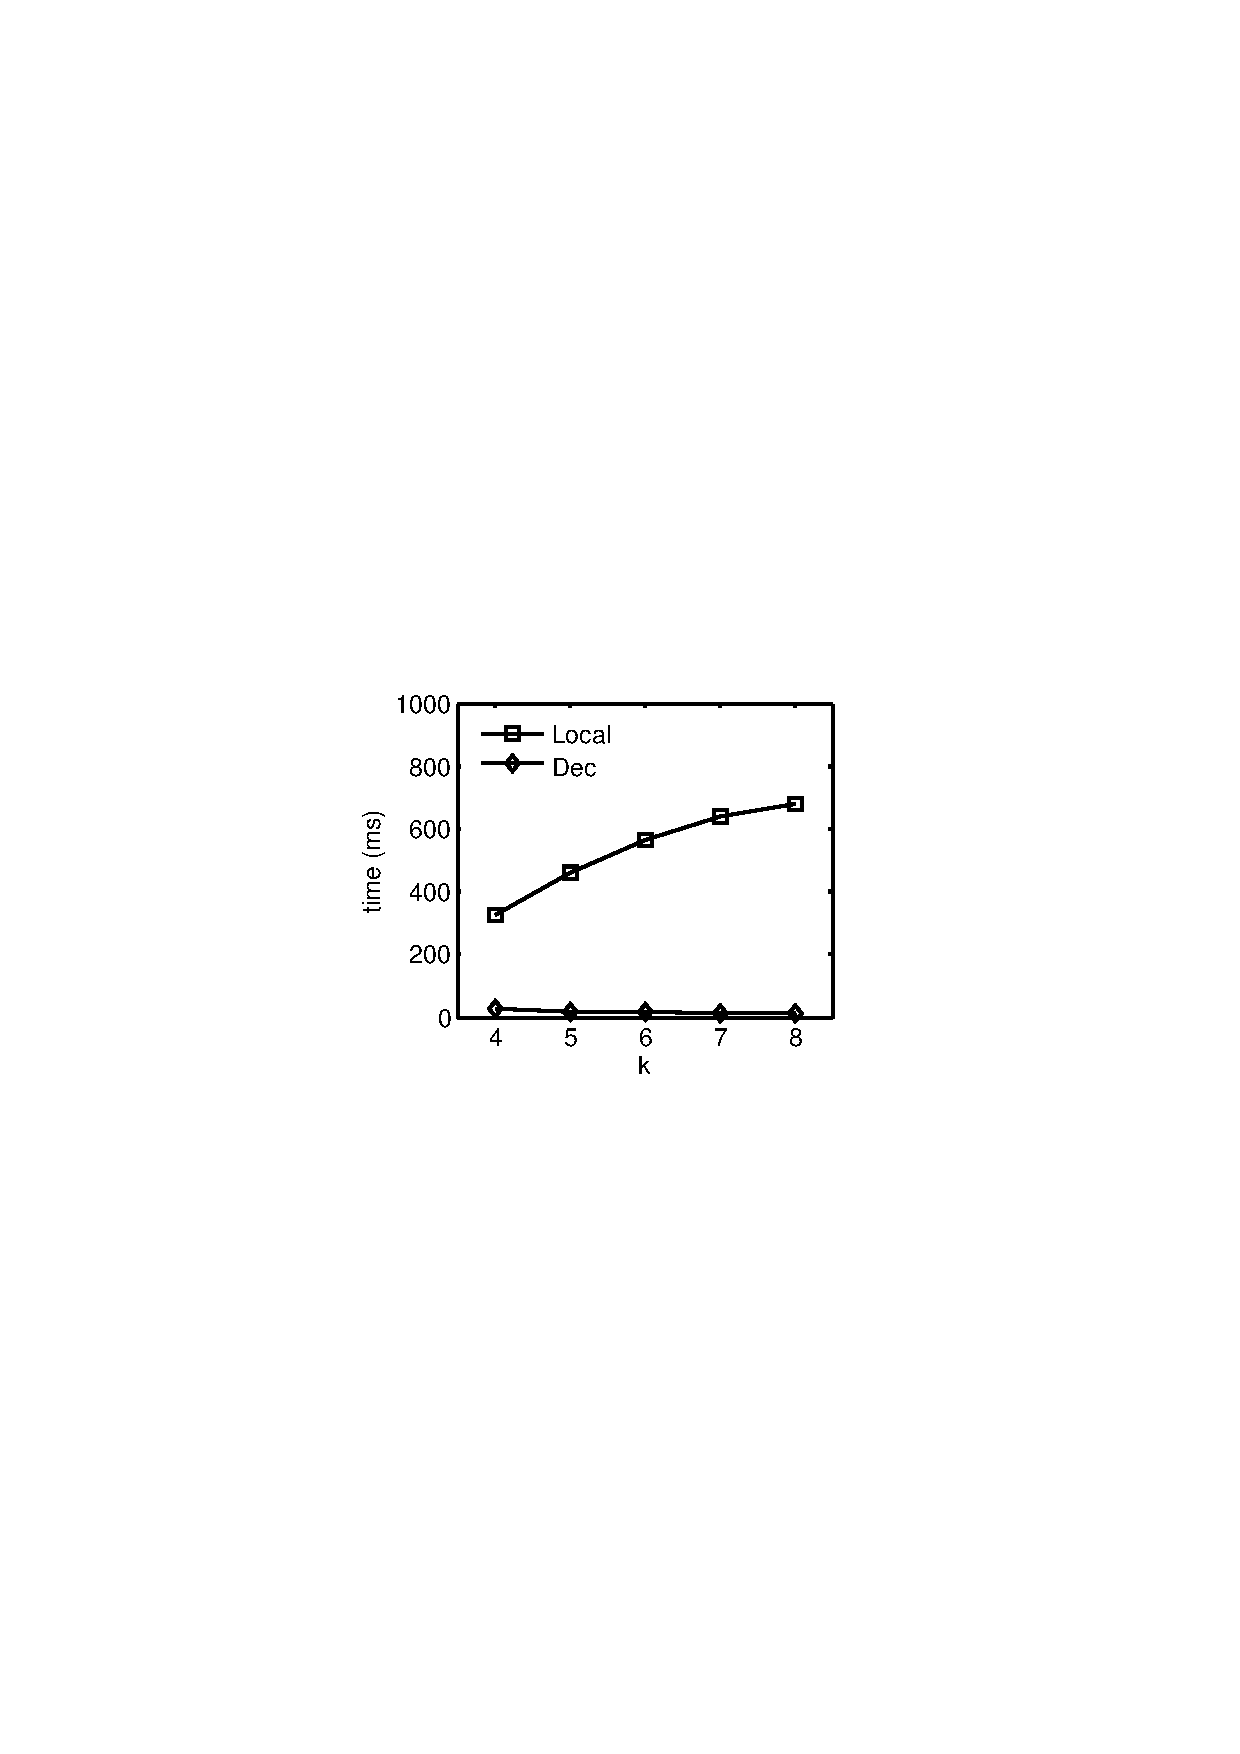
\includegraphics[width=3.325cm]{figures/flickrDecComp}
  \end{minipage}
  &
  \begin{minipage}{3.36cm}
	\includegraphics[width=3.325cm]{figures/dblpDecComp}
  \end{minipage}
  &
  \begin{minipage}{3.36cm}
	\includegraphics[width=3.325cm]{figures/tencentDecComp}
  \end{minipage}
  &
  \begin{minipage}{3.36cm}
	\includegraphics[width=3.325cm]{figures/dbpediaDecComp}
  \end{minipage}
  \\
  \small (a) Flickr
  &
  \small (b) DBLP
  &
  \small (c) Tencent
  &
  \small (d) DBpedia
\end{tabular}
\caption{Results on non-attributed graphs.}
\label{fig:exp-more-decComp}
\end{figure*}



\begin{figure*}[htb]
\hspace*{-.4cm}
\centering
\begin{tabular}{c c c c}
  \begin{minipage}{3.325cm}
  \includegraphics[width=3.725cm]{figures/flickrv1}
  \end{minipage}
  &
  \begin{minipage}{3.325cm}
  \includegraphics[width=3.725cm]{figures/dblpv1}
  \end{minipage}
  &
  \begin{minipage}{3.325cm}
  \includegraphics[width=3.725cm]{figures/tencentv1}
  \end{minipage}
  &
  \begin{minipage}{3.325cm}
  \includegraphics[width=3.725cm]{figures/dbpediav1}
  \end{minipage}
  \\
  \small (a) Flickr (Variant 1)
  &
  \small (b) DBLP (Variant 1)
  &
  \small (c) Tencent (Variant 1)
  &
  \small (d) DBpedia (Variant 1)
      \\
  \begin{minipage}{3.325cm}
  \includegraphics[width=3.725cm]{figures/flickrv2}
  \end{minipage}
  &
  \begin{minipage}{3.325cm}
  \includegraphics[width=3.725cm]{figures/dblpv2}
  \end{minipage}
  &
  \begin{minipage}{3.325cm}
  \includegraphics[width=3.725cm]{figures/tencentv2}
  \end{minipage}
  &
  \begin{minipage}{3.325cm}
  \includegraphics[width=3.725cm]{figures/dbpediav2}
  \end{minipage}
  \\
  \small (e) Flickr (Variant 2)
  &
  \small (f) DBLP (Variant 2)
  &
  \small (g) Tencent (Variant 2)
  &
  \small (h) DBpedia (Variant 2)
\\


\end{tabular}
\caption{Efficiency results of Variants of ACQ problem.}
\label{fig:exp-variant}
\end{figure*}


\textbf{8. Effect of invertedList.}
To test the importance of invertedList, we have implemented {\tt Inc-S*} and {\tt Inc-T*}, which are respective variants of {\tt Inc-S} and {\tt Inc-T}, but without the invertedList structure at each CL-tree node. Figure~\ref{fig:exp-more-inverted} shows the results. We see that {\tt Inc-S} ({\tt Inc-T}) is 1 to 2 order of magnitude faster than {\tt Inc-S*} ({\tt Inc-T*}) on all the four datasets in our experiments.
The reason is that the keyword-checking operation mentioned in the above example is frequently performed in the ACQ search process. Thus, the invertedList, which improves the performance of this operation, allows the ACQ search to be conducted more efficiently.

\textbf{9. Non-attributed graphs.}
We have tested {\tt Dec} and {\tt Local} on non-attributed graphs. This is done by running these algorithms on our datasets, without using any of their associated keyword sets. As shown in Figure~\ref{fig:exp-more-decComp}, for Flickr, Tencent and DBpedia, {\tt Dec} is consistently faster than {\tt Local}. In {\tt Dec}, cores are organized into the CL-tree structure. Because the height of the CL-tree is not very high (lower than 405 for all datasets), the core-locating operation can be done quickly. For DBLP, {\tt Dec} is also  faster than {\tt Local}, except when $k$=4. In this dataset, a paper often has few (around 3 to 5) co-authors. Since an author may be closely related to a few co-authors, finding a 4-$\widehat {core}$ in {\tt Local} can be done efficiently through local expansion.  From these experiments, we conclude that {\tt Dec} can also be efficiently executed on non-attributed graphs.

{\color{blue}
\textbf{10. Effect of $\theta$ in Variant 1.}
For each query vertex, we randomly select 10 keywords to form set $S$, set $\theta$ as 0.2, 0.4 0.6, 0.8 and 1.0,
and answer the query of Variant 1 using {\tt basic-g-v1}, {\tt basic-w-v1} and {\tt SWT}.
Figures~\ref{fig:exp-variant}(a)-\ref{fig:exp-variant}(d) show their efficiency.
We can see that {\tt SWT} outperforms the basic solutions consistently, as it uses the CL-tree index.

\textbf{11. Effect of $|Q|$ in Variant 2.}
We randomly select five groups of query sets by varying the size of $Q$ from 2 to 6.
Each group has 200 query sets.
We run {\tt basic-g-v2}, {\tt basic-w-v2} and {\tt MDec} with these five groups of query sets,
and report efficiency in Figures~\ref{fig:exp-variant}(e)-\ref{fig:exp-variant}(h).
Similar to the results of single query vertices, we can observe that {\tt MDec} is at least two orders of magnitude faster than the baseline solutions which do not use the CL-tree index.
}

%\chen{
%\subsection{Experiments on Variants}
%\label{app:varExp}
%\chen{
%The experimental results of variants are presented here and the basic algorithms for these variants are attached in Appendix~\ref{app:algoOfVariant}.
%}
%
%\textbf{1. Case study of Variants 1 and 2.}
%We search Jiawei Han's communities with explicit AC-label constraints in Variants 1 and 2.
%We consider two keyword sets, \textit{i.e.}, $S_1$=$\{$stream, classification$\}$ and $S_2$=$\{$cube, information, cluster$\}$.
%Note that the captions indicate the shared keywords of the communities.
%While for Variant 1 ($\theta$=0.6), we can obtain two communities (see Figures~\ref{fig:jiawei-v1}(a) and~\ref{fig:jiawei-v1}(b)). This implies that, for Variant 1, although we cannot find a community with AC-label being exactly $S_2$, we still can find a community, in which each member contains at least 60\% percentage of keywords of the input query keyword set. And for Variant 2, if the query set is \{Jiawei Han, Jing gao\}, and the keyword set is $S_1$=$\{$stream, classification$\}$, we will also obtain the community in Figures~\ref{fig:jiawei-v1}(a).
%
%
%\begin{figure}[ht]
%    \centering
%    \mbox{
%        \subfigure[$\{$stream, classification$\}$]{
%            \includegraphics[width=.42\columnwidth]{figures/jiawei-v1-1}
%            \label{fig:jiawei-v1-1}
%        }
%        \hspace{1ex}
%        \subfigure[$\{$cube, information$\}$]{
%            \includegraphics[width=.415\columnwidth]{figures/jiawei-v1-2}
%            \label{fig:jiawei-v1-2}
%        }
%    }
%    \caption{Jiawei Han's communities on Variants 1 and 2.}\label{fig:jiawei-v1}
%\end{figure}
%
%
%
%
%\textbf{2. Effect of $\theta$ in Variant 1.}
%For each query vertex, we randomly select 10 keywords to form set $S$, set $\theta$ as 0.2, 0.4 0.6, 0.8 and 1.0,
%and answer the query of Variant 1 using {\tt basic-g-v1}, {\tt basic-w-v1} and {\tt SWT}.
%Figures~\ref{fig:exp-variant}(a)-\ref{fig:exp-variant}(d) show their efficiency.
%We can see that {\tt SWT} outperforms the basic solutions consistently, as it uses the CL-tree index.
%
%{\color{blue}
%\textbf{3. Effect of $|Q|$ in Variant 2.}
%We limit query vertices with no more than 6 keywords.
%We randomly select 2, 3, 4, 5, 6 vertices to form the query set, and answer the query of Variant 2 using {\tt basic-g-v2}, {\tt basic-w-v2} and {\tt MDec}. Figures~\ref{fig:exp-variant}(e)-\ref{fig:exp-variant}(h) show their efficiency. Similar with Variant 2, we can see that {\tt MDec} performs the best by using the CL-tree index.
%}
%
%}  

\section{Conclusions}
\label{conclusion}

An AC is a community that exhibits structure and keyword cohesiveness. To facilitate ACQ evaluation, we develop the CL-tree index and its query algorithms. We further propose index maintenance algorithms for dynamic graphs.
Moreover, we formally define ACQ-A and ACQ-M problems and propose efficient query algorithms based on the CL-tree index.
Our experimental results on several dataseats show that ACs are easier to interpret than those of existing community detection/search methods, and they can be ``personalized''. In addition, our solutions are also faster than existing community search algorithms.

In the future, we will study the use of other measures of structure cohesiveness (e.g., $k$-truss, $k$-clique) and keyword cohesiveness (e.g., Jaccard similarity and string edit distance) in the ACQ definition.
We will also investigate how the directions of edges will affect the formation of an AC.
We will examine how graph pattern matching techniques \cite{GPM-KDD2007,GPM-VLDB2010,GPM-PVLDB2015} can be extended to find ACs effectively from large attributed graphs. An interesting research direction is to study how to automatically generate a meaningful graph pattern that well reflects a real community, and how to use these patterns to find ACs efficiently. 

\section*{Acknowledgments}
Reynold Cheng, Yixiang Fang, Siqaing Luo, and Jiafeng Hu were supported by the Research Grants Council of Hong Kong (RGC Project HKU 17205115) and HKU (Project 104004129).
%We would like to thank the reviewers for their insightful comments.

\bibliographystyle{abbrv}
\vspace{0.99em}
\small{\bibliography{lac}}
%\bibliography{lac}

%\bibliographystyle{abbrv}
%{\scriptsize
%\bibliography{lac}
%}

%\appendix

\section{Proofs of Lemmas}
\label{app:proof}

% go back to the original orders
\addtocounter{lemma}{-1}
\addtocounter{lemma}{-1}
\addtocounter{lemma}{-1}
\addtocounter{lemma}{-1}
\addtocounter{equation}{-1}
\addtocounter{equation}{-1}

\begin{lemma}[Anti-monotonicity]
  \label{lemma:apriori-app}
  Given a graph $G$, a vertex $q\in G$ and a set $S$ of keywords, if there exists a subgraph $G_k[S]$,
  then there exists a subgraph $G_k[S']$ for any subset $S'\subseteq S$.
\end{lemma}

\begin{proof}
Based on the definition of $G_k[S]$, each vertex of $G_k[S]$ contains $S$.
Consider a new keyword set $S'\subseteq S$.
We can easily conclude that,
each vertex of $G_k[S]$ contains $S'$ as well.
Also, note that $q\in G_k[S]$.
These two properties imply that there exists one subgraph of $G$,
namely $G_k[S]$, with core number at least $k$,
such that it contains $q$ and every vertex of it contains keyword set $S'$.
It follows that there exists such a subgraph with maximal size (\textit{i.e.}, $G_k[S']$).
\end{proof}

\begin{proposition}\label{prop:pre-app}
  For any keyword set $S$, and vertex $q$,
  if $G_k[S]$ exists, then $G_k[S]\subseteq G_k[S']$ for any subset $S'\subseteq S$.
\end{proposition}

\begin{proof}
Since $G_k[S]$ contains vertex $q$ and every vertex in $G_k[S]$ contains $S'$ (due to $S'\subseteq S$), then $G_k[S]\cup G_k[S']$ also contains vertex $q$ and every vertex in it contains $S'$. In addition, the core numbers of $G_k[S]$ and $G_k[S']$ are at least $k$, it follows that the core number of $G_k[S]\cup G_k[S']$ is at least $k$.
Based on the definition of $G_k[S']$, we have $G_k[S]\cup G_k[S']\subseteq G_k[S']$. It follows that $G_k[S]\subseteq G_k[S']$.
\end{proof}


\begin{lemma}
\label{lemma:coreDown-app}
  Given two subgraphs $G_k[S_1]$ and $G_k[S_2]$ of a graph $G$,
  for a new keyword set $S'$ generated from $S_1$ and $S_2$ (\textit{i.e.}, $S'=S_1\cup S_2$),
  if $G_k[S']$ exists, then it must appear in a $k$-$\widehat {core}$ with core number at least
  \begin{equation}
    max\{core_G[G_k[S_1]], core_G[G_k[S_2]]\}.
  \end{equation}
\end{lemma}

\begin{proof}
Since $S'$ is generated from $S_1$ and $S_2$, then $S_1\subseteq S'$ and $S_2 \subseteq S'$. Based on Proposition~\ref{prop:pre-app}, we have $G_k[S']\subseteq G_k[S_1]$. With such a containment relationship, it follows that $min\{core_G[v]|$ $v\in G_k[S_1]\}\leq min\{core_G[v]|v\in G_k[S']\}$. Hence, the core number of $G_k[S']$ is at least the core number of $G_k[S_1]$. Formally, $core_G[G_k[S_1]]$ $\leq core_G[G_k[S']]$. For the same reason, $core_G[G_k[S_2]]\leq core_G[G_k[S']]$. It directly follows the lemma.
\end{proof}



\begin{lemma}
\label{lemma:coreExist-app}
  Given a connected graph $G(V,E)$ with $n$=$|V|$ and $m$=$|E|$,
  if $m - n < \frac{{{k^2} - k}}{2} - 1$, there is no $k$-$\widehat {core}$ in $G$.
\end{lemma}

\begin{proof}
From Definition~\ref{def:kcore}, we can easily conclude that,
for any specific $k$, a $k$-$\widehat {core}$ has at least $k$+1 vertices.
Since each vertex in a specific $k$-$\widehat {core}$ has at least $k$ edges,
the minimum number of edges in a $k$-$\widehat {core}$ is $\frac{{(k + 1)k}}{2}$.

Consider a connected graph, which contains a $k$-$\widehat {core}$ and has the minimum number of edges,
where the $k$-core contains only $k+1$ vertices and
all the rest $n-(k+1)$ vertices are connected with this $k$-$\widehat {core}$.
The total number of edges is
\begin{equation}
\frac{{(k + 1)k}}{2} + \left[ {n - (k + 1)} \right] = m
\end{equation}

By simple transformation, we can conclude that,
if $m - n < \frac{{{k^2} - k}}{2} - 1$, there is no $k$-$\widehat {core}$ in $G$.
\end{proof}



\begin{lemma}
\label{lemma:kcoreIntersect-app}
  Given two keyword sets $S_1$ and $S_2$, if $G_k[S_1]$ and $G_k[S_2]$ exist, we have
  \begin{equation}
    G_k[S_1\cup S_2] \subseteq G_k[S_1]\cap G_k[S_2].
  \end{equation}
\end{lemma}

\begin{proof}
Based on Proposition~\ref{prop:pre-app} and $S_1\subseteq {S_1} \cup {S_2}$, we have ${G_k}[{S_1} \cup {S_2}]\subseteq {G_k}[{S_1}]$. For the same reason we have ${G_k}[{S_1} \cup {S_2}]\subseteq {G_k}[{S_2}]$. It directly follows the lemma.
\end{proof}


\section{Basic Solutions for ACQ}
\label{app:basic}

Algorithms~\ref{alg:basic-g} and~\ref{alg:basic-w} present {\tt basic-g} and {\tt basic-w} respectively.
The input of {\tt basic-g} is a graph $G$, a query vertex $q$, an integer $k$ and a set $S$.
It first generates a set, $\Psi$, of candidate keyword sets,
each of which contains a single keyword of $S$ (line 2).
Then, it finds the $k$-$\widehat {core}$, ${\mathcal C}_k$, containing $q$ from the graph $G$.
In the while loop (lines 4-14), it first initializes an empty set $\Phi$ (line 5),
which is used to collect all the qualified keyword sets.
Then for each candidate keyword set $S'\in \Psi$,
it finds $G[S']$ from ${\mathcal C}_k$ by considering the keyword constraint.
After that, it finds $G_k[S']$ from $G[S']$ (lines 7-8),
and put it into $\Phi$ if $G_k[S']$ exists (lines 9-10).
After checking all the candidate keyword sets in $\Psi$,
if there are at least one qualified keyword sets in $\Phi$,
it generates a new set $\Psi$ of larger candidate keyword sets
by calling \textsc{geneCand($\Phi$)} (see Appendix~\ref{app:geneCand})
and continues to checking longer candidate keyword sets in next loop;
otherwise, it stops and outputs all the communities of the latest verified keyword sets as the target ACs.


\begin{algorithm}[h]
\caption{Basic solution: {\tt basic-g}}
\label{alg:basic-g}
\footnotesize{
\algrenewcommand{\algorithmiccomment}[1]{\hskip3em$//$ #1}
\begin{algorithmic}[1]
    \Function{query($G$, $q$, $k$, $S$)}{}
        \State init $\Psi$ using $S$;
        \State find the $k$-$\widehat {core}$, ${\mathcal C}_k$, containing $q$ from $G$;
        \While {true}
            \State $\Phi\gets \emptyset$;
            \For {each $S'$ $\in \Psi$}
                \State find $G[S']$ from ${\mathcal C}_k$;
                \State find $G_k[S']$ from $G[S']$;
                \If {$G_k[S']$ exists}
                    \State $\Phi$.add($S'$);
                \EndIf
            \EndFor
            \If {$\Phi \ne \emptyset$}
                \State $\Psi\gets$ \Call{geneCand($\Phi$)}{};
            \Else
                \State break;
            \EndIf
        \EndWhile
        \State output the communities of keyword sets in $\Phi$;
    \EndFunction
\end{algorithmic}}
\end{algorithm}

Algorithm~\ref{alg:basic-w} presents the pseudocodes of {\tt basic-w}.
It follows the main steps of {\tt basic-g},
except that for each candidate keyword set $S'$,
it finds $G[S']$ from $G$ directly,
rather than from ${\mathcal C}_k$.

\begin{algorithm}[h]
\caption{Basic solution: {\tt basic-w}}
\label{alg:basic-w}
\footnotesize{
\algrenewcommand{\algorithmiccomment}[1]{\hskip3em$//$ #1}
\begin{algorithmic}[1]
    \Function{query($G$, $q$, $k$, $S$)}{}
        \State init $\Psi$ using $S$;
        \While {true}
            \State $\Phi\gets \emptyset$;
            \For {each $S'$ $\in \Psi$}
                \State find $G[S']$ from $G$;
                \State find $G_k[S']$ from $G[S']$;
                \If {$G_k[S']$ exists}
                    \State $\Phi$.add($S'$);
                \EndIf
            \EndFor
            \If {$\Phi \ne \emptyset$}
                \State $\Psi\gets$ \Call{geneCand($\Phi$)}{};
            \Else
                \State break;
            \EndIf
        \EndWhile
        \State output the communities of keyword sets in $\Phi$;
    \EndFunction
\end{algorithmic}}
\end{algorithm}


\section{Candidate Generation}
\label{app:geneCand}

Given a set $\Phi$ of qualified keyword sets,
Algorithm~\ref{alg:geneCand} generates new candidate keyword sets incrementally
by linking each pair of keyword sets.
We first initialize $\Psi$ as an empty set (line 2).
Then for each pair, $S_i$ and $S_j$, of keyword sets in $\Phi$,
we sort their keywords.
If they differ only at the last keyword,
then we generate a new keyword set $S'$=$S_i\cup S_j$,
by a union operation (lines 3-6).
According to Lemma~\ref{lemma:apriori},
if any subset of $S'$ does not appear in $\Phi$, we prune $S'$;
otherwise, we regard it as a candidate and add it into $\Psi$ (lines 7-8).
Finally, we return $\Psi$ as the results (line 9).

\begin{algorithm}[h]
\caption{Generate candidate keyword sets}
\label{alg:geneCand}
\footnotesize{
\algrenewcommand{\algorithmiccomment}[1]{\hskip3em$//$ #1}
\begin{algorithmic}[1]
    \Function{geneCand($\Phi$)}{}
        \State $\Psi\gets \emptyset$;
        \For {each $S_i$ $\in \Phi$}
            \For {each $S_j$ $\in \Phi$}
                \If {$S_i$ and $S_j$ differs at the last keyword}
                    \State initialize $S'$=$S_i\cup S_j$;
                    \If {$S'$ cannot be pruned by Lemma~\ref{lemma:apriori}}
                        \State $\Psi$.add($S'$);
                    \EndIf
                \EndIf
            \EndFor
        \EndFor
        \State \Return $\Psi$;
    \EndFunction
\end{algorithmic}}
\end{algorithm}


\section{Anchored Union-find}
\label{app:auf}

Algorithm~\ref{alg:unionFindAppendix} presents
the four functions of the anchored union-find (AUF) data structure.
\begin{algorithm}[h]
\caption{Functions on the AUF data structure}
\label{alg:unionFindAppendix}
\footnotesize{
\algrenewcommand{\algorithmiccomment}[1]{\hskip3em$//$ #1}
\begin{algorithmic}[1]
    \Function{makeSet($x$)}{}
        \State $x.parent, x.anchor\gets x$;
        \State $x.rank\gets 0$;
    \EndFunction
    \Function{find($x$)}{}
        \If {$x.parent$=$x$}
            \State $x.parent\gets$ \Call{find($x.parent$)}{};
        \EndIf
        \State \Return $x.parent$;
    \EndFunction
    \Function{union($x$, $y$)}{}
        \State $xRoot\gets$  \Call{find($x$)}{};
        \State $yRoot\gets$  \Call{find($y$)}{};
        \If {$xRoot$=$yRoot$}
            \Return;
        \EndIf
        \If {$xRoot.rank<yRoot.rank$}
            \State $xRoot.parent\gets yRoot$;
        \ElsIf {$xRoot.rank>yRoot.rank$}
            \State $yRoot.parent\gets xRoot$;
        \Else
            \State $yRoot.parent\gets xRoot$;
            \State $xRoot.rank\gets xRoot.rank$ + 1;
        \EndIf
    \EndFunction
    \Function{updateAnchor($x$, $core_G[\text{ }]$, $y$)}{}
        \State $xRoot\gets$ \Call{find($x$)}{};
        \If {$core_G[xRoot.anchor]>core_G[y]$}
            \State $xRoot.anchor\gets y$;
        \EndIf
    \EndFunction
\end{algorithmic}}
\end{algorithm}

The functions \textsc{find} and \textsc{union} are exactly the same
as that of the classical union-find data structure~\cite{unionFind}.
For function \textsc{makeSet}, the only change made on the classical \textsc{makeSet}
is that, it initializes $x.anchor$ as $x$ (line 2).
The function \textsc{updateAnchor} is used to update the anchor vertex of $x$'s representative vertex.
It first finds $x$'s representative vertex by calling \textsc{find} (line 20).
Then, if the core number of $x$' representative vertex is larger than that of the current input vertex $y$,
it updates the anchor vertex of $x$'s representative vertex as $y$.

\textbf{Complexity analysis.}
The time complexities of functions \textsc{find} and \textsc{union} are $O(\alpha(n))$~\cite{unionFind},
where $\alpha(n)$ is less than 5 for all practical values of $n$.
In function \textsc{makeSet}, 
the time complexity of \textsc{makeSet} is still $O(1)$.
In function \textsc{updateAnchor}, as \textsc{find} can be completed in $O(\alpha(n))$
and updating anchor can be completed in $O(1)$,
the total time cost of function \textsc{updateAnchor} is $O(\alpha(n))$. 

\section{Basic Algorithms for Variants}
\label{app:algoOfVariant}

{\color{blue}
\textbf{1. Variant 1.}
We present {\tt basic-g-v1} and {\tt basic-w-v1} in Algorithms~\ref{alg:basic-g-v1} and~\ref{alg:basic-w-v1} respectively.

\begin{algorithm}[h]
\caption{Query algorithm: {\tt basic-g-v1}}
\label{alg:basic-g-v1}
\footnotesize{
\algrenewcommand{\algorithmiccomment}[1]{\hskip3em$//$ #1}
\begin{algorithmic}[1]
    \Function{query($G$, $q$, $k$, $S$)}{}
        \State find the $k$-$\widehat {core}$, ${\mathcal C}_k$, containing $q$ from $G$;
        \State collect a set $V'$ of vertices containing at least $|S|\times \theta$ keywords from ${\mathcal C}_k$;
        \State find $G[S]$ from the subgraph induced by $V'$;
        \State find $G_k[S]$ from $G[S]$;
        \State output $G_k[S]$ as the target AC.
    \EndFunction
\end{algorithmic}}
\end{algorithm}

\begin{algorithm}[h]
\caption{Query algorithm: {\tt basic-w-v1}}
\label{alg:basic-w-v1}
\footnotesize{
\algrenewcommand{\algorithmiccomment}[1]{\hskip3em$//$ #1}
\begin{algorithmic}[1]
    \Function{query($G$, $q$, $k$, $S$)}{}
        \State collect a set $V'$ of vertices containing at least $|S|\times \theta$ keywords from $G$;
        \State find $G[S]$ from the subgraph induced by $V'$;
        \State find $G_k[S]$ from $G[S]$;
        \State output $G_k[S]$ as the target AC.
    \EndFunction
\end{algorithmic}}
\end{algorithm}

\textbf{2. Variant 2.}
Algorithms {\tt basic-g-v2}, {\tt basic-w-v2} are extended from {\tt basic-g} and {\tt basic-w}.
Detailed pseudocodes are attached in Algorithms~\ref{alg:basic-g-v2} and~\ref{alg:basic-w-v2} respectively.

\begin{algorithm}[h]
\caption{Query algorithm: {\tt basic-g-v2}}
\label{alg:basic-g-v2}
\footnotesize{
\algrenewcommand{\algorithmiccomment}[1]{\hskip3em$//$ #1}
\begin{algorithmic}[1]
    \Function{query($G$, $Q$, $k$, $S$)}{}
        \State $S'$ = $( \bigcap_{i=0}^{|Q|-1}W(q_i))\cap S$;
        \State $q \gets$ randomly select a vertex from $Q$;
        \State run {\tt basic-g} with $q$, $k$, and $S'$;
        \State output target ACs which contain $Q$;
    \EndFunction
\end{algorithmic}}
\end{algorithm}
\vspace{-0.6cm}
\begin{algorithm}[h]
\caption{Query algorithm: {\tt basic-w-v2}}
\label{alg:basic-w-v2}
\footnotesize{
\algrenewcommand{\algorithmiccomment}[1]{\hskip3em$//$ #1}
\begin{algorithmic}[1]
    \Function{query($G$, $Q$, $k$, $S$)}{}
        \State $S$ = $( \bigcap_{i=0}^{|Q|-1}W(q_i))\cap S$;
        \State $q \gets$ randomly select a vertex from $Q$;
        \State run {\tt basic-w} with $q$, $k$, and $S'$;
        \State output target ACs which contain $Q$;
    \EndFunction
\end{algorithmic}}
\end{algorithm}
} 

\end{document}
